\chapter{Partie technique}

Après avoir établi l'IS de notre projet, nous nous sommes lancés dans la réalisation technique au deuxième semestre.

La partie programme de notre système se divise en deux parties. La première, le "détecteur", permet de détecter les pupilles, de déplacer le curseur et de cliquer. La seconde partie, l’interface graphique, propose à l’utilisateur une IHM simplifiée, composée des fonctionnalités qui lui seront les plus utiles. Ce sera l’OS, ici Windows ou MAC, qui permet le lien entre ces deux parties du système. En effet, le détecteur permet de déplacer le curseur et de cliquer sur l’interface graphique.

\section{Le détecteur}

La partie "détecteur" de notre système permet de déplacer le curseur et de cliquer grâce au mouvement oculaire. Comme nous pouvons le voir figure \ref{fig:ESDetecteur}, le détecteur prend en entrée un flux vidéo acquis par la webcam et permet d’agir, en déplaçant le curseur et cliquant, sur l’interface graphique. 

\begin{figure}[H]
  \centering
  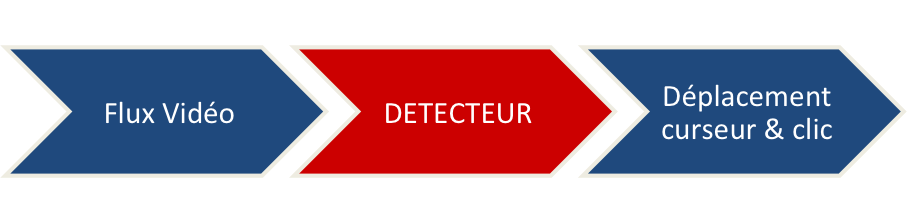
\includegraphics[scale=1]{ESDetecteur}
  \caption{Entrée/Sortie du détecteur}
  \label{fig:ESDetecteur}
\end{figure}

\subsection{Principe de fonctionnement}

Le détecteur est composé de différentes parties que nous pouvons retrouver sous forme de méthodes (voir figure \ref{fig:OrganisationDetecteur}). Ces différentes parties permettent de :

\begin{enumerate}
\item Acquérir le flux vidéo et le transformer en images matricielles
\item Détecter le visage
\item Détecter les yeux
\item Déterminer le centre des pupilles
\item Déplacer le curseur en fonction de la position des centres
\item Cliquer
\end{enumerate}

Afin d’expliquer comment sont réalisées ces fonctionnalités, nous allons présenter rapidement différentes méthodes qui composent le détecteur en nous attardant sur les points essentiels vus ci-dessus.

D’autre part, il est important de signaler que nous avons essayé de convertir la position du centre de la pupille en coordonnée de curseur de différentes façons. Ainsi, il existe plusieurs versions informatiques du détecteur. Dans la suite de cette partie du rapport, nous présenterons les méthodes les plus claires afin de faciliter la compréhension du lecteur. Cependant, suivant la version du détecteur, ces méthodes pourront présenter quelques différences.

\begin{figure}[H]
  \centering
  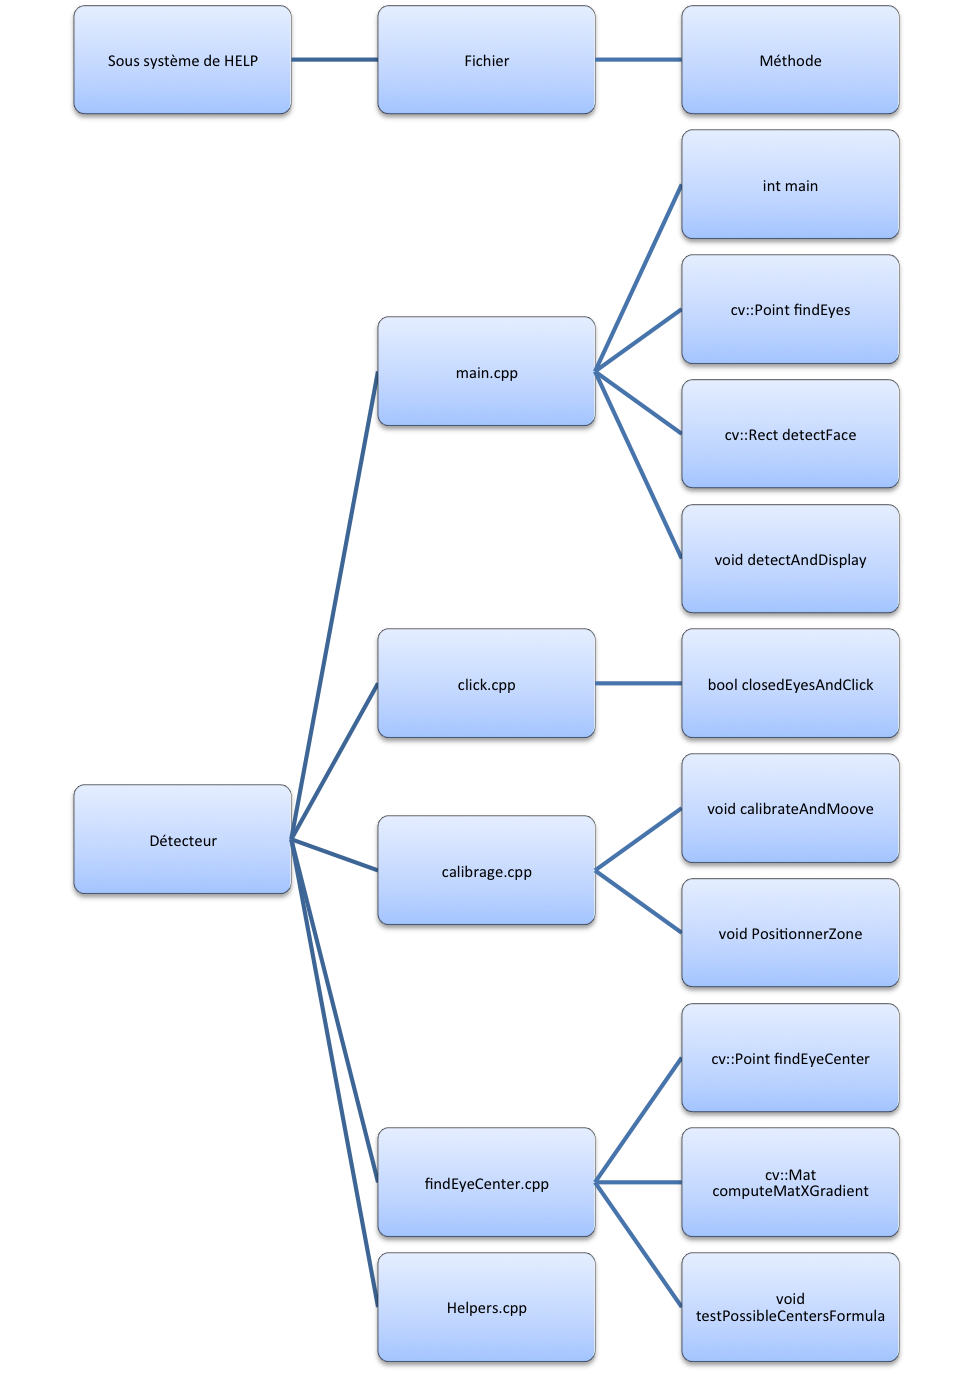
\includegraphics[scale=0.8]{OrganisationDetecteur}
  \caption{Organisation du détecteur}
  \label{fig:OrganisationDetecteur}
\end{figure}

\subsection{Acquisition du flux vidéo et transformation en images matricielles}

La méthode main permet de récupérer le flux vidéo et de le convertir en images matricielles (voir annexe \ref{A2}). Ces images matricielles seront nécessaires aux méthodes utilisées par le détecteur. La méthode \lstinline=cvCaptureFromCam(0)= permet de récupérer le flux vidéo de la webcam 0. Ensuite, dans une boucle \lstinline=while=, l’image matricielle, récupérée grâce à la méthode \lstinline=cvQueryFrame=, est inversée selon la verticale grâce à la méthode \lstinline=cv::flip= afin de faciliter l’utilisation des méthodes du détecteur. En effet, sans cette inversion, un mouvement vers la droite de l’utilisateur correspondrait à un mouvement vers la gauche sur l’écran de l’ordinateur. Ainsi, cette inversion facilite par exemple le placement de l’utilisateur.

\subsection{Détection du visage}

Tout d’abord, il faut savoir que nous effectuons la détection du visage et des yeux grâce aux haar\_cascades  \cite{lienhart2002extended}\cite{viola2001rapid}.

\paragraph{Haar\_cascades / Caractéristiques pseudo-Haar}

Les caractéristiques pseudo-Haar (Haar-like features en anglais) sont utilisées en vision par ordinateur pour détecter des objets dans des images numériques. Le principal avantage de celles-ci est la rapidité de calcul. Cependant, la simplicité de ces caractéristiques permettant cette rapidité de calcul impose une détection d’objets simples. Ces caractéristiques sont des fenêtres de détection (ou masques) qui délimitent des zones rectangulaires adjacentes. Une caractéristique rectangulaire simple peut être définie comme la différence des sommes de pixels de deux ou plusieurs zones rectangulaires adjacentes. De plus, ce rectangle prend toutes les tailles possibles et se déplace à toutes les positions de l’image à laquelle est appliquée cette caractéristique. Les valeurs indiquent certaines caractéristiques d’une zone particulière de l’image. \textbf{Une caractéristique est donc un nombre réel qui code les variations du contenu pixellique à une position et taille donnée dans la fenêtre de détection.} Chaque type de caractéristique peut indiquer l’existence (ou l’absence) de certaines caractéristiques dans l’image étudiée telles que des contours ou des changements de texture. Par exemple, une caractéristique à 2 rectangles permet d’indiquer où se situe une frontière entre une zone sombre et une zone claire.

\begin{figure}[H]
  \centering
  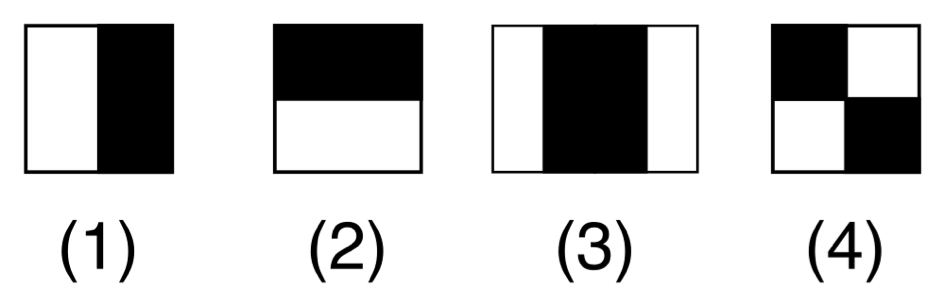
\includegraphics[scale=0.8]{pseudoHaar}
  \caption{Un exemple des premières caractéristiques pseudo-Haar utilisées par Viola et Jones en 2001 \\Source : Indif - Wikimedia Commons}
  \label{fig:pseudoHaar}
\end{figure}

Ensuite, un classifieur est crée à partir de quelques centaines d’images de l’objet ciblé (dans notre cas, le visage et les yeux). Ces images sont dimensionnées à la même taille et sont en négatif. Une fois le classifieur créé, il peut être appliqué à une région d’une image selon la méthode précédemment vue. Ainsi, il sera retourné un nombre réel proche de 1 lorsque la région ciblée de l’image sera proche du classifieur et 0 lorsqu’elle s’en éloignera. Pour rechercher l’objet dans toute l’image, le classifieur sera déplacé à travers toute l’image étudiée. De plus, il sera redimensionné afin de trouver l’objet recherché à différentes tailles (ce qui est plus simple que de redimensionner l’image elle-même). 

Le mot "cascade" dans le nom du classifieur signifie que le classifieur résultant se compose de plusieurs classifieurs simples (étapes) qui sont appliqués à la suite à une région d’intérêt jusqu’à ce que, à un moment donné, la région candidate soit rejetée ou ait passé toutes les étapes. Le mot "boosté" signifie que les classifieurs, à chaque étape de la cascade, sont eux-mêmes complexes et qu’ils sont construits sur des classifieurs de base en utilisant l'une des quatre techniques différentes suivantes : Discrete Adaboost, Real Adaboost, Gentle Adaboost and Logitboost. Les caractéristiques pseudo-haar sont l’entrée du classifieur basique.

\paragraph{Utilisation de ces haar\_cascades}

La méthode \lstinline=detectFace= permet de réaliser la détection du visage grâce à un haar\_cascade. Elle prend en entrée l’image acquise par la webcam. Les haar\_cascades permettant de détecter le visage et les yeux sont d’abord chargés dans le main (voir annexe \ref{A3}) puis, dans la méthode \lstinline=detectFace=, un vecteur de rectangles est créé et rempli lors de l’utilisation de l’haar\_cascade. Dans cette matrice se trouvent donc les rectangles encadrant le visage (voir annexe \ref{A4}). La méthode trace ensuite un rectangle (voir figure \ref{fig:DetectionVisage}) autour du visage en prenant le premier rectangle de ce vecteur. La méthode \lstinline=detectFace= retourne ce rectangle.

\begin{figure}[H]
  \centering
  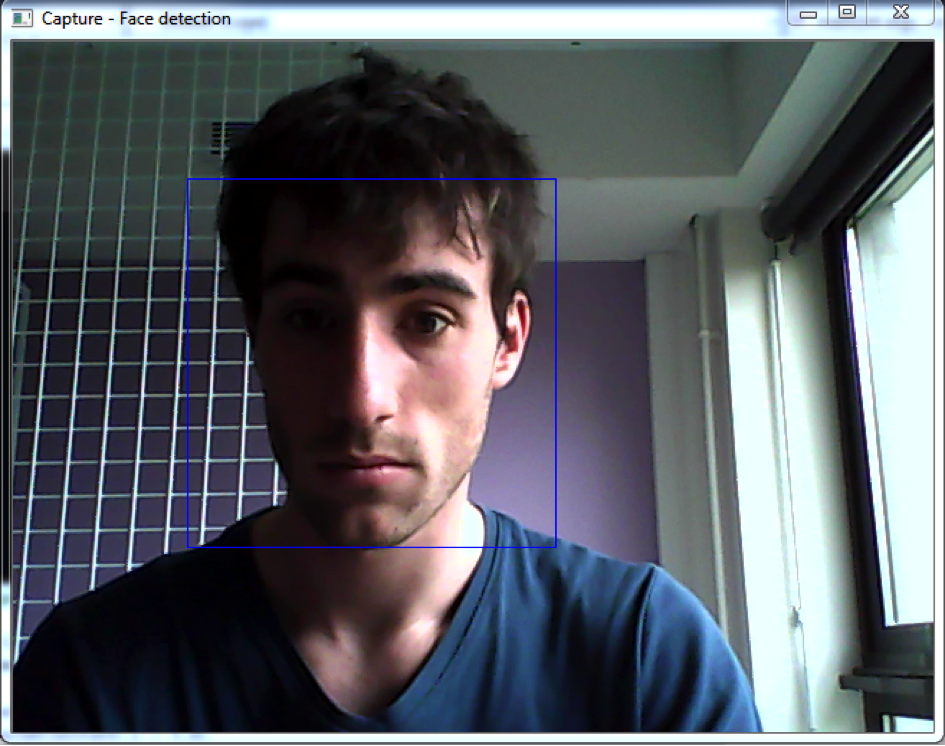
\includegraphics[scale=0.8]{DetectionVisage}
  \caption{Détection du visage}
  \label{fig:DetectionVisage}
\end{figure}

\subsection{Détection des yeux}

La méthode \lstinline=closedEyesAndClick= qui prend en argument l’image du visage ainsi que l’haar\_cascade permettant de détecter un œil, et qui retourne un booléen en fonction de l’ouverture ou non de l’œil, permet de détecter l’œil. En effet, de la même manière que pour la détection du visage, un vecteur "eyes" contenant les rectangles encadrant les yeux est créé. Ensuite, la méthode \lstinline=detectMultiScale= permet de remplir ce vecteur grâce à l’image du visage et l’haar\_cascade (voir annexe \ref{A5}).

\subsection{Détermination du centre des pupilles}

Concernant la détection du centre des pupilles, la méthode \lstinline=findEyeCenter= prend en argument une matrice contenant l’image du visage, un rectangle encadrant l’œil et un nom de fenêtre dans laquelle sera affichée l’image de l’œil traitée par la méthode. Tout d’abord, dans cette méthode, le rectangle encadrant l’œil appliqué à l’image du visage permet de créer une matrice contenant l’image de l’œil. Ce sera grâce à cette matrice que sera détecté le centre des pupilles. De plus, la méthode retourne les coordonnées, dans l’image de l’œil, du centre des pupilles. Il sera ensuite effectué un changement de repères dans la méthode \lstinline=findEyes= afin de d’obtenir les coordonnées des pupilles dans l’image du visage (voir figure \ref{fig:centrePupilles} et annexe \ref{A6}).

\begin{figure}[H]
  \centering
  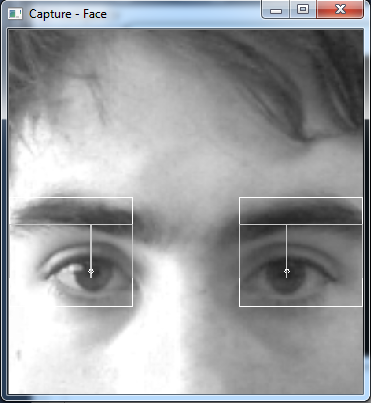
\includegraphics[scale=0.8]{centrePupilles}
  \caption{Détection du centre des pupilles}
  \label{fig:centrePupilles}
\end{figure}

\paragraph{Localisation du centre des pupilles}

Afin de localiser le centre des pupilles, nous avons utilisé un code de Tristan Hume \cite{eyelike} qui s’appuie sur un article de Fabian Timm \cite{timm2011accurate}. Cet article décrit une méthode s’appuyant sur les gradients. La direction de ces gradients est utilisée afin de déterminer le centre des pupilles. Cependant, dans l’image de l’œil, plusieurs centres des pupilles sont possibles si l’on considère seulement les gradients. En effet, certains facteurs tels que les sourcils, les paupières, des lunettes, ou tout simplement des reflets peuvent modifier la valeur théorique des gradients et ainsi, plusieurs centres sont possibles.

Considérons un centre possible $\mathbf{c}$ et un vecteur gradient $\mathbf{g}_i$ à la position $\mathbf{x}_i$. Le vecteur $\mathbf{d}_i$ de la distance normalisée (entre $\mathbf{c}$ et $\mathbf{x}_i$) devrait avoir la même orientation que $\mathbf{g}_i$. Ainsi, le produit scalaire entre ces deux vecteurs devrait être égale à un. Pour trouver le centre optimal $\mathbf{c}*$ des pupilles, il faudrait donc que la somme sur i des produits scalaires entre $\mathbf{d}_i$ et $\mathbf{g}_i$ soit maximale. Ainsi, $c*$ sera égale à l'argument du maximum sur $\mathbf{c}$, noté $arg \max$, (l'ensemble des points en lesquels une expression atteint sa valeur maximale) de cette somme.

\begin{equation}
\mathbf{c}* = arg\max_{\mathbf{c}}\left (\frac{1}{N}\sum_{i=1}^N(\mathbf{d}_i^T\mathbf{g}_i)^2\right )
\label{eq:1}
\end{equation}

\begin{equation}
\mathbf{d}_i = \frac{\mathbf{x}_i - \mathbf{c}}{\left \| \mathbf{x}_i - \mathbf{c} \right \|_2} , \forall i : \|\mathbf{g}_i\|_2 = 1
\label{eq:2}
\end{equation}

Nous pouvons voir une illustration de cette méthode figure \ref{fig:schemaAlgoCentrePupilles}.

\begin{figure}[H]
  \centering
  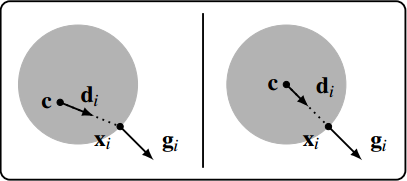
\includegraphics[scale=1]{schemaAlgoCentrePupilles}
  \caption{Exemple de localisation du centre d'un rond noir sur fond blanc \cite{timm2011accurate}}
  \label{fig:schemaAlgoCentrePupilles}
\end{figure}

\paragraph{Algorithme du gradient}

Concernant l’algorithme utilisé afin de calculer les gradients dans l’image de l’œil. L’algorithme utilisé par la méthode \lstinline=findEyeCenter= est celui utilisé par Matlab transformé en C++. En Matlab, cela donne \lstinline=[x(2)-x(1) (x(3:end)-x(1:end-2))/2 x(end)-x(end-1)=], avec \lstinline=x= l’entrée (voir annexe \ref{A7} pour la version en C++ utilisée par \lstinline=findEyeCenter=). Le gradient \lstinline=X= est ainsi obtenu comme suit \lstinline-cv::Mat gradientX = computeMatXGradient(eyeROI)- et le gradient \lstinline=Y= est obtenu en tranposant le résultat de la méthode appliquée à la transposée de \lstinline=X= : \lstinline-cv::Mat gradientY = computeMatXGradient(eyeROI.t()).t()-
Ensuite, un seuil est appliqué grâce à la méthode \lstinline=computeDynamicThreshold= afin de filtrer les gradients obtenus \lstinline-double gradientThresh = computeDynamicThreshold(mags, kGradientThreshold)- où "mags" est la matrice des magnitudes de tous les gradients calculés.

\subsection{Déplacement du curseur en fonction de la position des centres}

Cette fonctionnalité est assurée par la méthode \lstinline=calibrateAndMoove=  qui prend en argument la position du centre d’une pupille dans l’image de l’œil. Cette méthode ne retourne rien, mais permet de déplacer le curseur.

\lstinline=CalibrateAndMoove= est composée de cinq parties différentes, quatre consacrées à la calibration et une dernière permettant le déplacement du curseur une fois la calibration effectuée. Les trois premières étapes consistent à enregistrer la position du centre de la pupille lorsque l’utilisateur regarde en haut à gauche de l’écran, puis en haut à droite et enfin en bas à gauche. Ces positions sont stockées dans la matrice \lstinline=pointsMesuresReference[3]=. Ensuite, la quatrième étape permet d’effectuer un changement de repère, la position du centre de la pupille est transformée en position du curseur sur l’écran. Pour cela, nous avons choisis de considérer qu’il s’agit d’un changement de repère affine. Nous pouvons voir figure \ref{fig:calib} un schéma de l’écran avec les coordonnés de trois coins de l’écran dans le repère de l’écran lui-même et dans le repère de l’image de la pupille.

\begin{figure}[H]
  \centering
  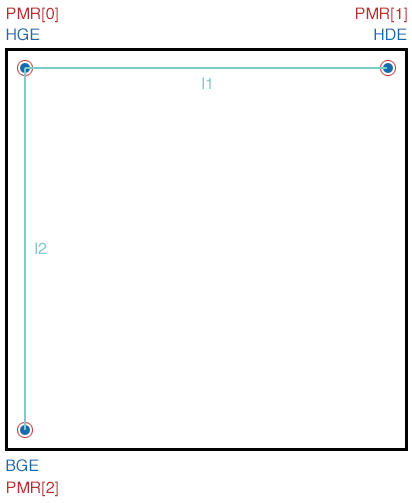
\includegraphics[scale=0.6]{Calibration}
  \caption{Schéma calibration}
  \label{fig:calib}
\end{figure}

Avec, entre autre :
\begin{itemize}[font=\tiny, label=\ding{108}]
\item \lstinline-PMR[0] = pointMesureReference[0]- qui correspond aux coordonnées de la pupille lorsque l’utilisateur regarde le coin en haut à gauche.
\item \lstinline-HGE = hautGaucheEcran- qui correspond au coordonnées du point en haut à gauche de l’écran (0,0).
\end{itemize}

Ainsi, la longueur l1 est égale à \lstinline=HGD.x= et correspond à \lstinline=(PMR[1]-PMR[0]).x=

Deux équations sont donc nécessaires à ce changement de repère (une suivant X et une suivant Y) et les coordonnée du point visé est calculé de la manière suivante :

\begin{lstlisting}
cv::Point pointVise;

		double aH = -(double)hautDroitEcran.x / (double)(pointsMesuresReference[0].x - pointsMesuresReference[1].x);
		double bH = (double)hautGaucheEcran.x - aH*pointsMesuresReference[0].x;

		double aV = -(double)basGaucheEcran.y / (double)(pointsMesuresReference[0].y - pointsMesuresReference[2].y);
		double bV = (double)hautGaucheEcran.y - aV*pointsMesuresReference[0].y;

		pointVise.x = aH*leftPupil.x + bH;
		pointVise.y = aV*leftPupil.y + bV;
\end{lstlisting}

Enfin, la cinquième partie permet de bouger le curseur grâce à \lstinline=SetCursorPos(pointVise.x, pointVise.y)=. De plus, la méthode  sera utilisée pour notre démonstrateur afin de découper l’écran en quatre zones (nous essaierons par la suite de découper en neuf zones). Ainsi, si le point visé se trouve dans la partie supérieure gauche de l’écran, le curseur sera placé au centre de cette zone (de même que pour les trois autres zones). 

\subsection{Clic}

Le clic est assuré par la méthode \lstinline=closedEyeAndClick= que nous avons déjà présenté précédemment. Lorsque l’œil n’est plus détecté (œil fermé) (détection de l’œil grâce à l’haar\_cascade), un compte à rebours est déclenché. Une fois l’œil rouvert, il est de nouveau détecté et le compte à rebours est stoppé. Si le délai est supérieur à 1 seconde et inférieur à 3 secondes, le clic est déclenché grâce à la fonction \lstinline=mouse_event=.

\begin{lstlisting}
mouse_event(MOUSEEVENTF_LEFTDOWN, 0, 0, 0, 0);
mouse_event(MOUSEEVENTF_LEFTUP, 0, 0, 0, 0);
\end{lstlisting}

\section{Interface graphique}

\subsection{But et enjeux de l’interface}

Dès le début du projet, l’idée d’une interface graphique permettant de contrôler le PC a été envisagée. En effet, la finalité est d’aider les personnes tétraplégiques, or, l’utilisation de l’interface standard d’un ordinateur reste compliquée. Nous avons donc pensé à créer notre propre outil de communication avec l'utilisateur, qui permettrait de lancer les programmes favoris de ce dernier.

\subsection{Critères d’exigence}

Afin de rendre l’IHM la plus ergonomique possible pour l’utilisateur, nous avons décidé de valider deux critères principaux. En premier lieu, l’interface devra être adaptée au contrôle via notre logiciel de gaze-tracking. Celui-ci étant parfois imprécis et pouvant être fatiguant à utiliser sur le long terme, nous avons fait en sorte que les boutons de l’interface occupent le maximum d’espace sur l’écran (voir figure \ref{fig:IG9B}).

\begin{figure}[H]
  \centering
  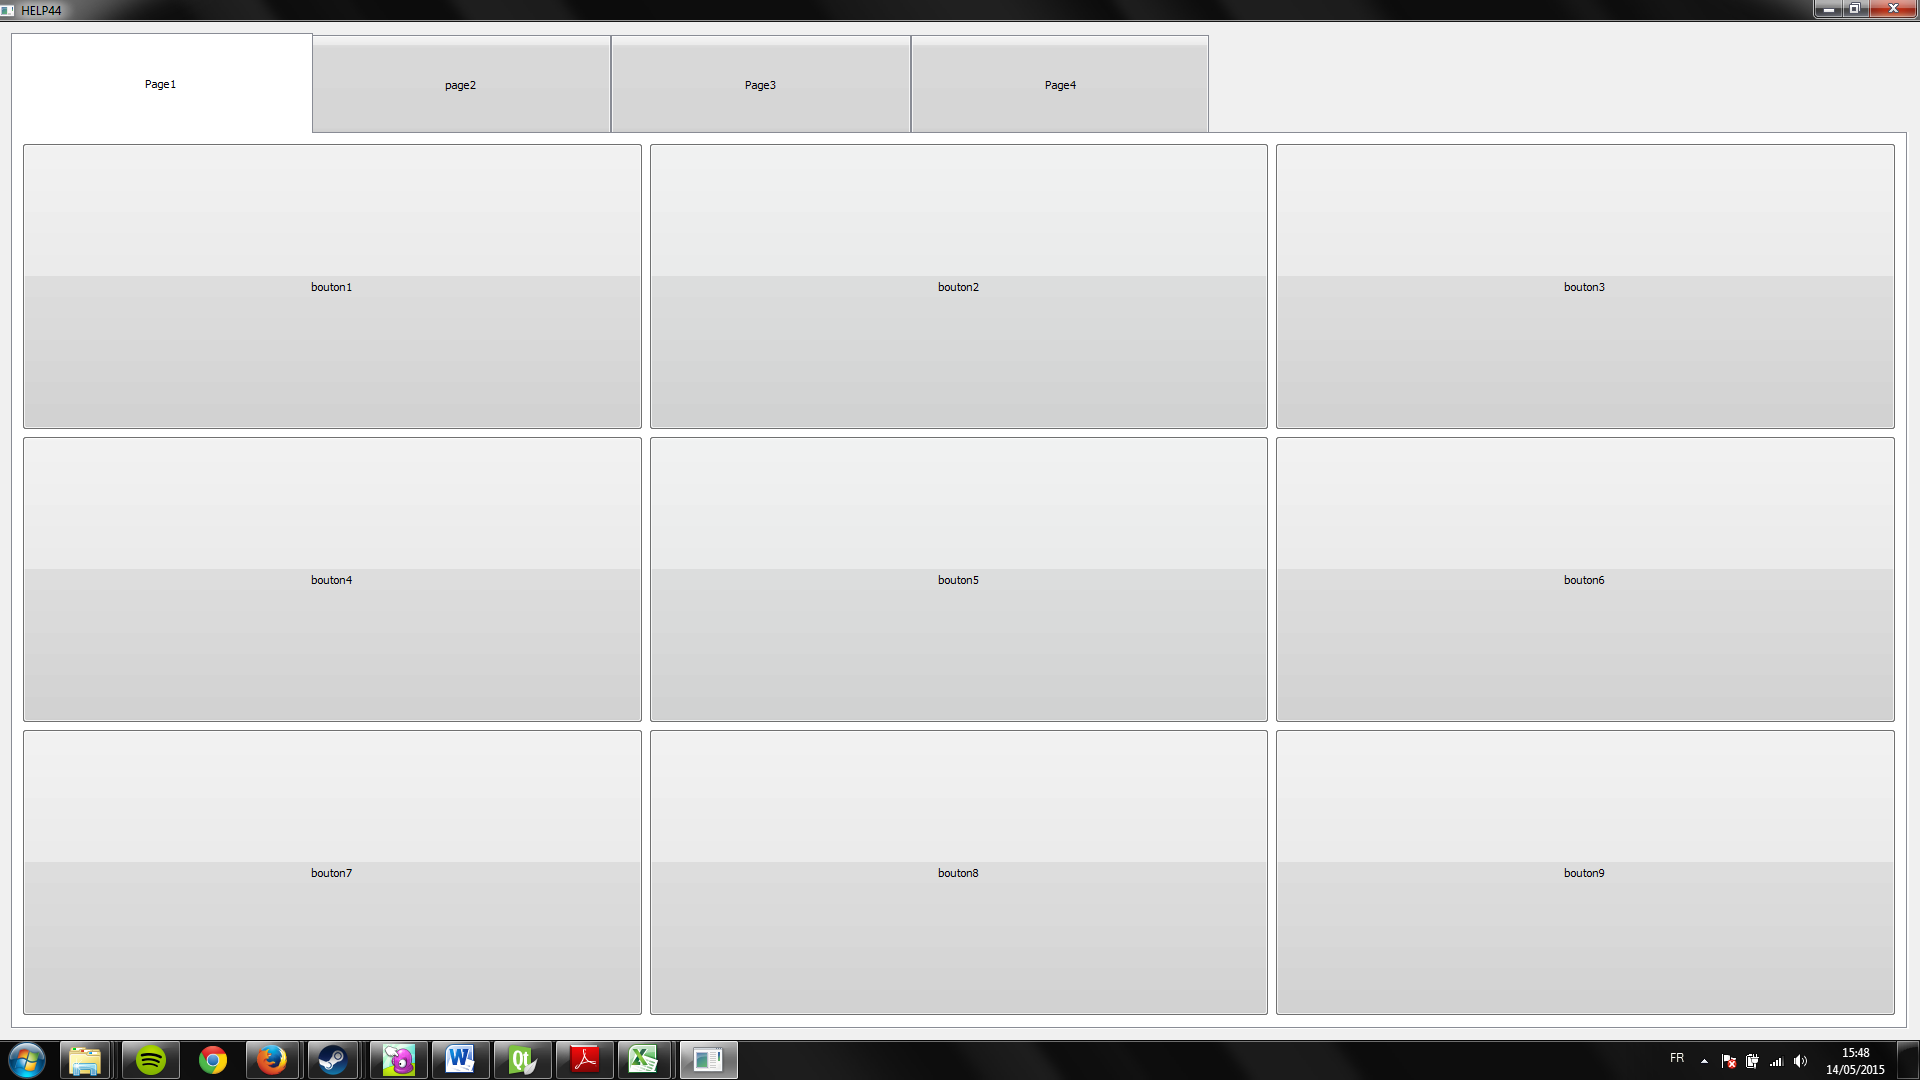
\includegraphics[scale=0.3]{IG9B}
  \caption{Interface graphique 9 boutons}
  \label{fig:IG9B}
\end{figure}

Deux modes de fonctionnement existent pour notre logiciel de gaze-tracking : un mode de fonctionnement libre, où l’utilisateur peut déplacer le curseur où il veut sur l’écran, et un mode assisté où le mouvement est restreint à certaines zones de l’écran. De plus, deux interfaces distinctes ont été développées. La première à neuf boutons (voir figure \ref{fig:IG9B}), réservée aux utilisateurs les plus à l’aise avec le logiciel de gaze-tracking et la seconde à quatre boutons (voir figure \ref{fig:IG4B}) pour les utilisateurs débutants. Ces deux interfaces autorisent l’utilisation du mode assisté et du mode libre.

\begin{figure}[H]
  \centering
  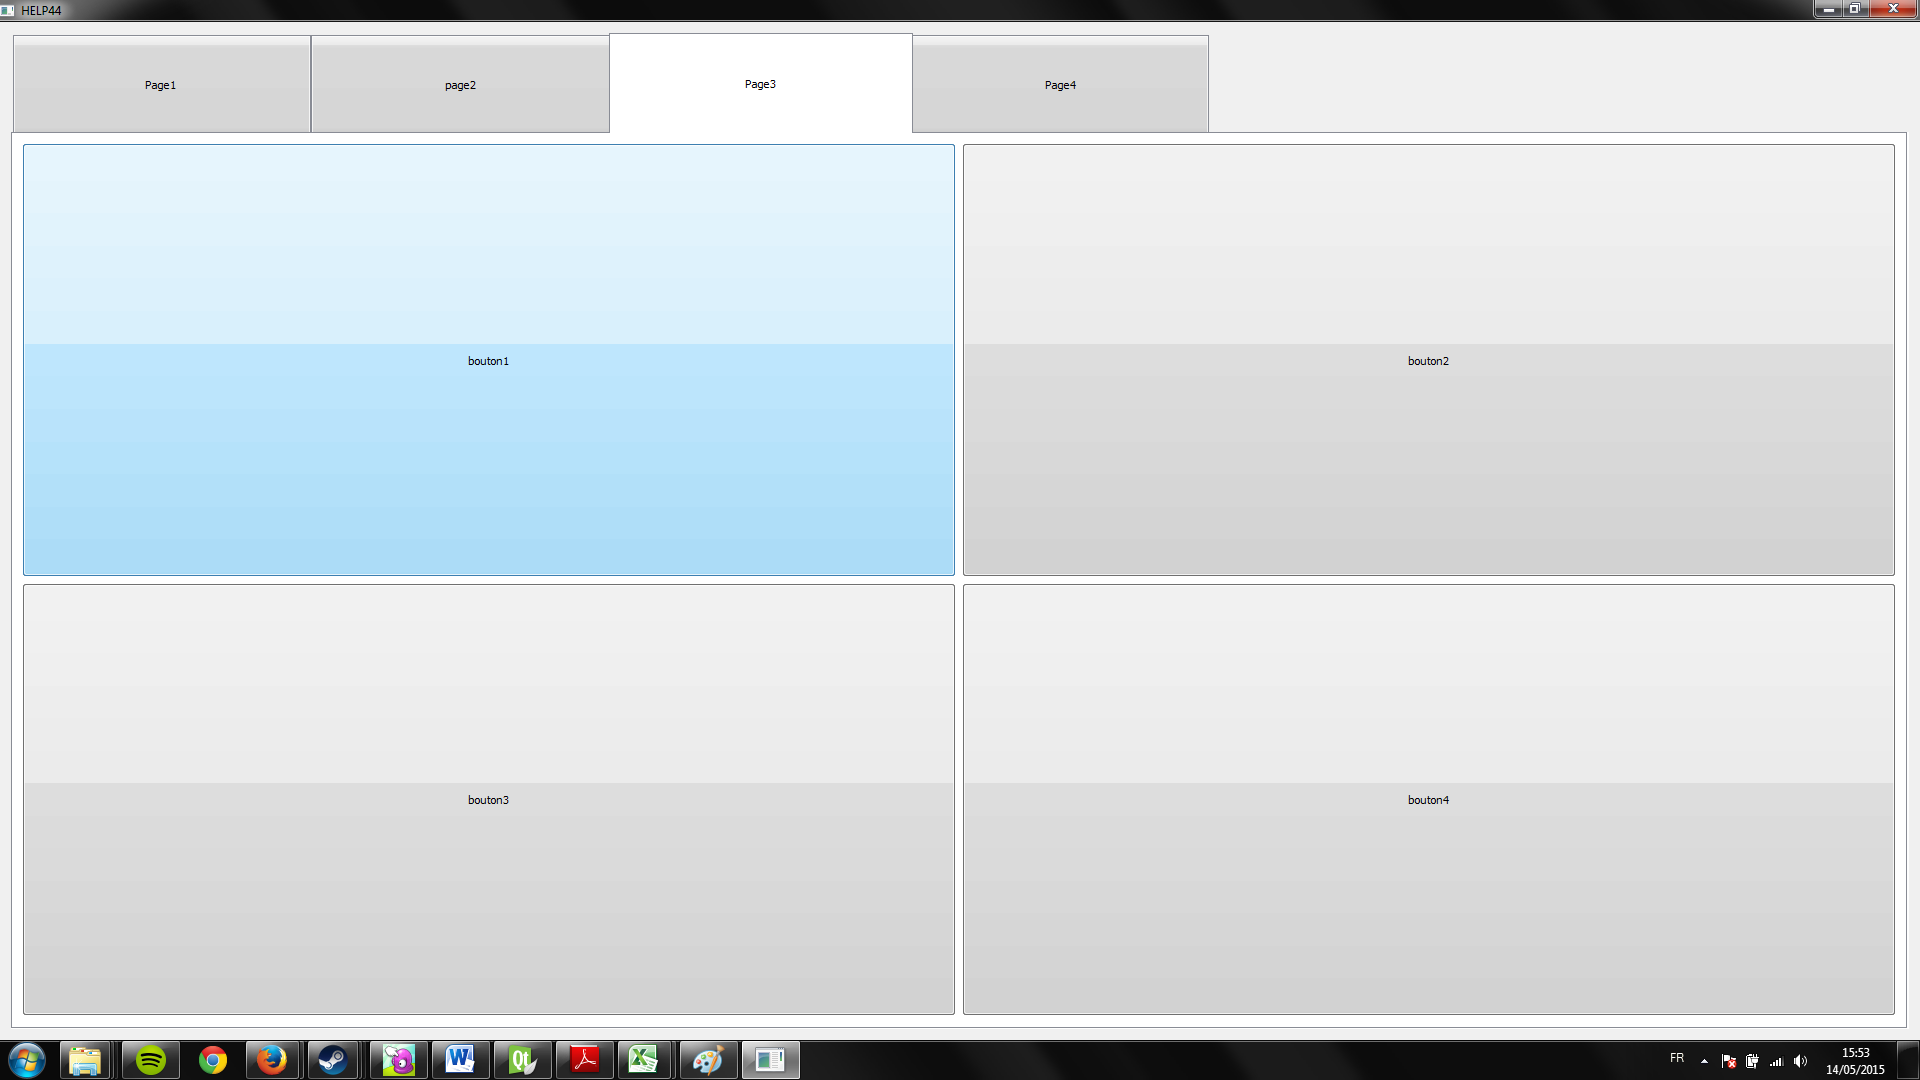
\includegraphics[scale=0.3]{IG4B}
  \caption{Interface graphique 4 boutons}
  \label{fig:IG4B}
\end{figure}

Dans un deuxième temps, l’interface devait être paramétrable afin de pouvoir lancer les logiciels favoris de l’utilisateur, ou encore un film ou un document PDF. Ainsi le clic sur l’un des boutons lance un logiciel, soit entré par défaut, soit personnalisable par l’utilisateur. La page permettant de paramétrer les boutons est présentée figure \ref{fig:IGconf9}.

\begin{figure}[H]
  \centering
  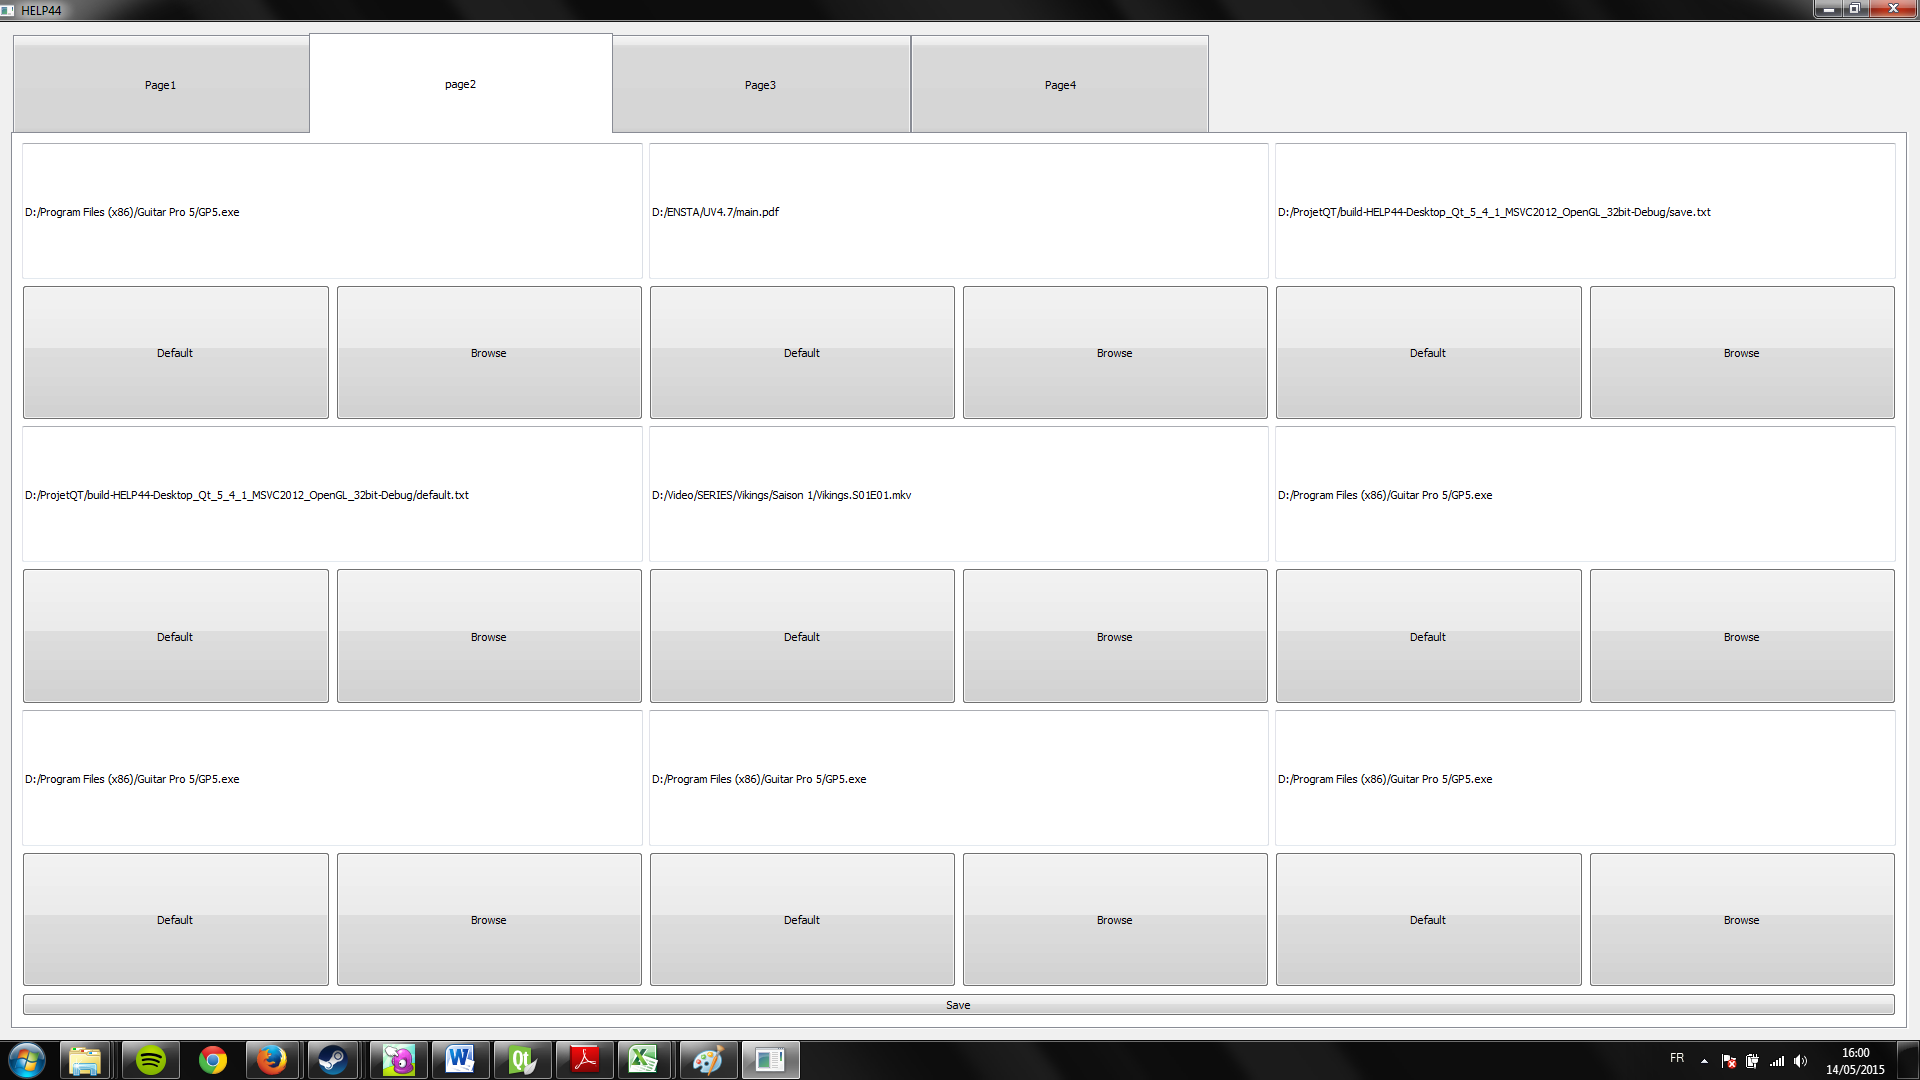
\includegraphics[scale=0.3]{IGconf9}
  \caption{Interface de configuration des 9 boutons (existe aussi pour les 4 boutons)}
  \label{fig:IGconf9}
\end{figure}

Chaque chemin peut être modifié à l’aide du bouton "Browse", qui permet de changer le logiciel exécuté par le bouton que l’on a choisi. Ces adresses peuvent ensuite être stockées dans un fichier texte à l’aide du bouton "Save" (le fichier texte se situe dans le dossier contenant l’exécutable). En cas d’erreur ou d’une manipulation non souhaitée, le bouton "Default" permet de lier de nouveau le bouton erroné à un chemin valide. Ces adresses par défaut permettent de lancer les logiciels d’ergonomie de Windows, ainsi que les utilitaires classiques tels que la calculatrice ou Internet Explorer.

\subsection{Outils de réalisation}

Comme langage de programmation, nous avons choisi le C++ couplé à Qt Creator, pour réaliser cette interface. En effet, notre programme de gaze-tracking étant codé en C++, il sera plus facile dans le futur de réunir les deux logiciels en un seul (chose qui n’est pas encore faite à ce jour). D’autre part la librairie Qt permet de faire rapidement et simplement des interfaces graphiques, et c’est donc présentée comme une évidence.

\section{Limites du système}

\subsection{Limites du détecteur}

Concernant les limites de la partie détecteur de notre système, nous pouvons distinguer trois grandes catégories :
\begin{itemize}[font=\tiny, label=\ding{108}]
\item Limites liées au mouvement de la tête
\item Limites liées à la caméra
\item Limites liées à la luminosité
\end{itemize}

\subsubsection{Limites liées au mouvement de la tête}

La principale limite de notre démonstrateur est l’absence de possibilité de mouvement de la tête. En effet, nous devons utiliser une mentonnière afin de maintenir la tête et de limiter les mouvements de celle-ci. Cette limite de notre démonstrateur peut s’expliquer par trois limites de notre système.

\paragraph{Limites des haar\_cascades}

La détection du centre des pupilles a d’abord été testée en utilisant l’image du visage où étaient récupérées les images des yeux grâce à des constantes liées à la morphologie du visage. Cependant, le rectangle encadrant le visage, renvoyé lors de l’utilisation de l’haar\_cascade permettant la détection du visage, n’est pas suffisamment précis. En effet, nous avons constaté un léger décalage de quelques pixels au cours du temps de ce rectangle (comme une vibration). Or, les coordonnées du centre des pupilles ayant une variation de seulement quelques pixels, ces décalages du rectangle modifiaient trop les coordonnées du centre pour avoir une estimation correcte du point visé sur l’écran. Nous avons donc essayé de récupérer l’image des yeux non plus grâce à des constantes, mais en utilisant un haar\_cascade permettant de récupérer le rectangle encadrant les yeux. Cependant, encore une fois, la position de ce rectangle variait trop au cours du temps. C’est pourquoi notre démonstrateur n’effectue pas cette détection du visage et film directement l’œil avec une tête sans mouvement.

\paragraph{Orientation de la tête}

Ensuite, une deuxième limite à notre système est qu’il ne prend pas en compte l’orientation de la tête. En effet, si le déplacement du visage dans le plan devrait être pris en compte, un mouvement circulaire de la tête vers la gauche ou la droite provoquerait un dérèglement du calibrage. En effet, lorsqu’un utilisateur fixe un point de l’écran en tournant la tête ou non, cela change les coordonnées du centre des pupilles. Cependant, nous pouvons penser qu’un utilisateur tétraplégique ne bougera pas sa tête, mais il ne faudra donc pas que sa tête glisse.

\paragraph{Tête verticale seulement}
La dernière limite quant  au mouvement de la tête est que l’haar\_cascade ne permet de détecter qu’un visage plus ou moins vertical. Empiriquement, nous avons vu qu’à partir d’un angle d’environ 10 degrés, l’haar\_cascade ne permettait plus la détection du visage. 

\subsubsection{Limites liées à la caméra}

Pour notre démonstrateur, nous utilisons une mentonnière afin de limiter les mouvements du visage qui induiraient de mauvaises valeurs pour les points visés. En effet, un décalage du visage par rapport à la caméra induirait un étalonnage obsolète. Ainsi, le principe du casque / lunettes étudié lors de la phase bibliographique aurait peut-être permis de pallier ce problème.

\subsubsection{Limites liées à la luminosité}

Une des principales limites de l’utilisation de la méthode permettant la détection du centre des pupilles est qu’elle s’appuie sur les gradients. Or, ces gradients peuvent être plus ou moins en accord avec leur valeur théorique selon la luminosité. En effet, un simple reflet dans la partie de l’image de la pupille peut avoir une influence assez conséquente sur la détermination de son centre. Si la méthode utilisée permet de réduire les défauts liés à ces aléas, les centres calculés restent parfois imprécis (hésitation entre deux positions par exemple). De plus, de part l’utilisation de la méthode des gradients, la méthode de détection du centre des pupilles est assez robuste avec des yeux clairs (yeux bleus), mais reste moins efficace avec les yeux sombres (yeux marrons).

\subsection{Limites d'utilisation}

\subsubsection{Limite d’utilisation pour l’utilisateur}

Les tests de validation fonctionnelle (un exemple de fiche complétée est donné en annexe \ref{AFV}) nous ont permis de mettre au clair plusieurs limitations concernant l’utilisateur de notre système. Tout d’abord, notre système reste encore trop fatigant lorsqu’il est utilisé en mode libre. En effet, les utilisateurs se sont vite fatigués à essayer de naviguer sur l’écran lorsque celui-ci n’est pas prédécoupé en différentes zones. La navigation est de plus encore difficile car trop imprécise.

D’un point de vue du confort, l’immobilité de la tête due à la mentonnière est aussi un point à améliorer. Cette immobilité forcée empêche l’utilisateur de parler ou de bouger la tête sous peine de devoir refaire une calibration. Le fait de fixer la mentonnière et l’ordinateur à la table pourrait aider à améliorer cette situation en offrant des repères parfaitement fixes.

Le champ de vision de l’utilisateur pose aussi un problème. Le fait de se concentrer sur une zone particulière de l’écran afin de cliquer dessus empêche la vision globale de l’écran.

La morphologie de l’utilisateur semble aussi très déterminante sur les résultats obtenus. Ainsi les yeux plus clairs semblent permettre un meilleur contrôle de la souris en comparaison aux yeux foncés. Certaines morphologies du visage rendent aussi la détection des yeux difficiles, et notamment lorsque l’utilisateur observe les angles de l’écran.

\subsubsection{Limite d’utilisation de l’interface graphique}

Concernant l’interface graphique, la principale limitation vient du fait qu’elle n’est encore totalement adaptée au contrôle avec notre logiciel. En effet le découpage de l’écran en différentes zones distinctes oblige à découper chaque onglet de façon différente. L’idéal serait donc de pouvoir faire abstraction de ce découpage et laisser un total contrôle à l’utilisateur. Cependant, la précision de notre logiciel ne le permet pas encore.

Une seconde limitation est liée à la personnalisation de notre interface. L’utilisateur ne peut pas configurer lui-même le nombre de bouton ou encore les placer où il veut à l’écran. De plus, dans le cadre ou l’utilisateur est tétraplégique, la personnalisation du logiciel lancé par un bouton donné devra forcément être faite par une tierce personne.

A l’heure actuel notre interface ne permet pas de lancer deux logiciels en même temps ce qui pose problème pour le multi-tasking. Cependant ce problème pourra facilement être corrigé dans les versions futures.

La dernière limitation vient du fait que même si notre interface permet facilement de lancer un logiciel, celui-ci doit aussi être utilisable à l’aide du gaze-tracking. Or la majorité des logiciels les plus courants ne possèdent pas de telles options. Il faudrait donc créer un lot de logiciel adapté à cette utilisation et notamment dans le cas où l’utilisateur est tétraplégique.